%% Two column figure below
\begin{figure*}[htbp]
%% Size
\centerline{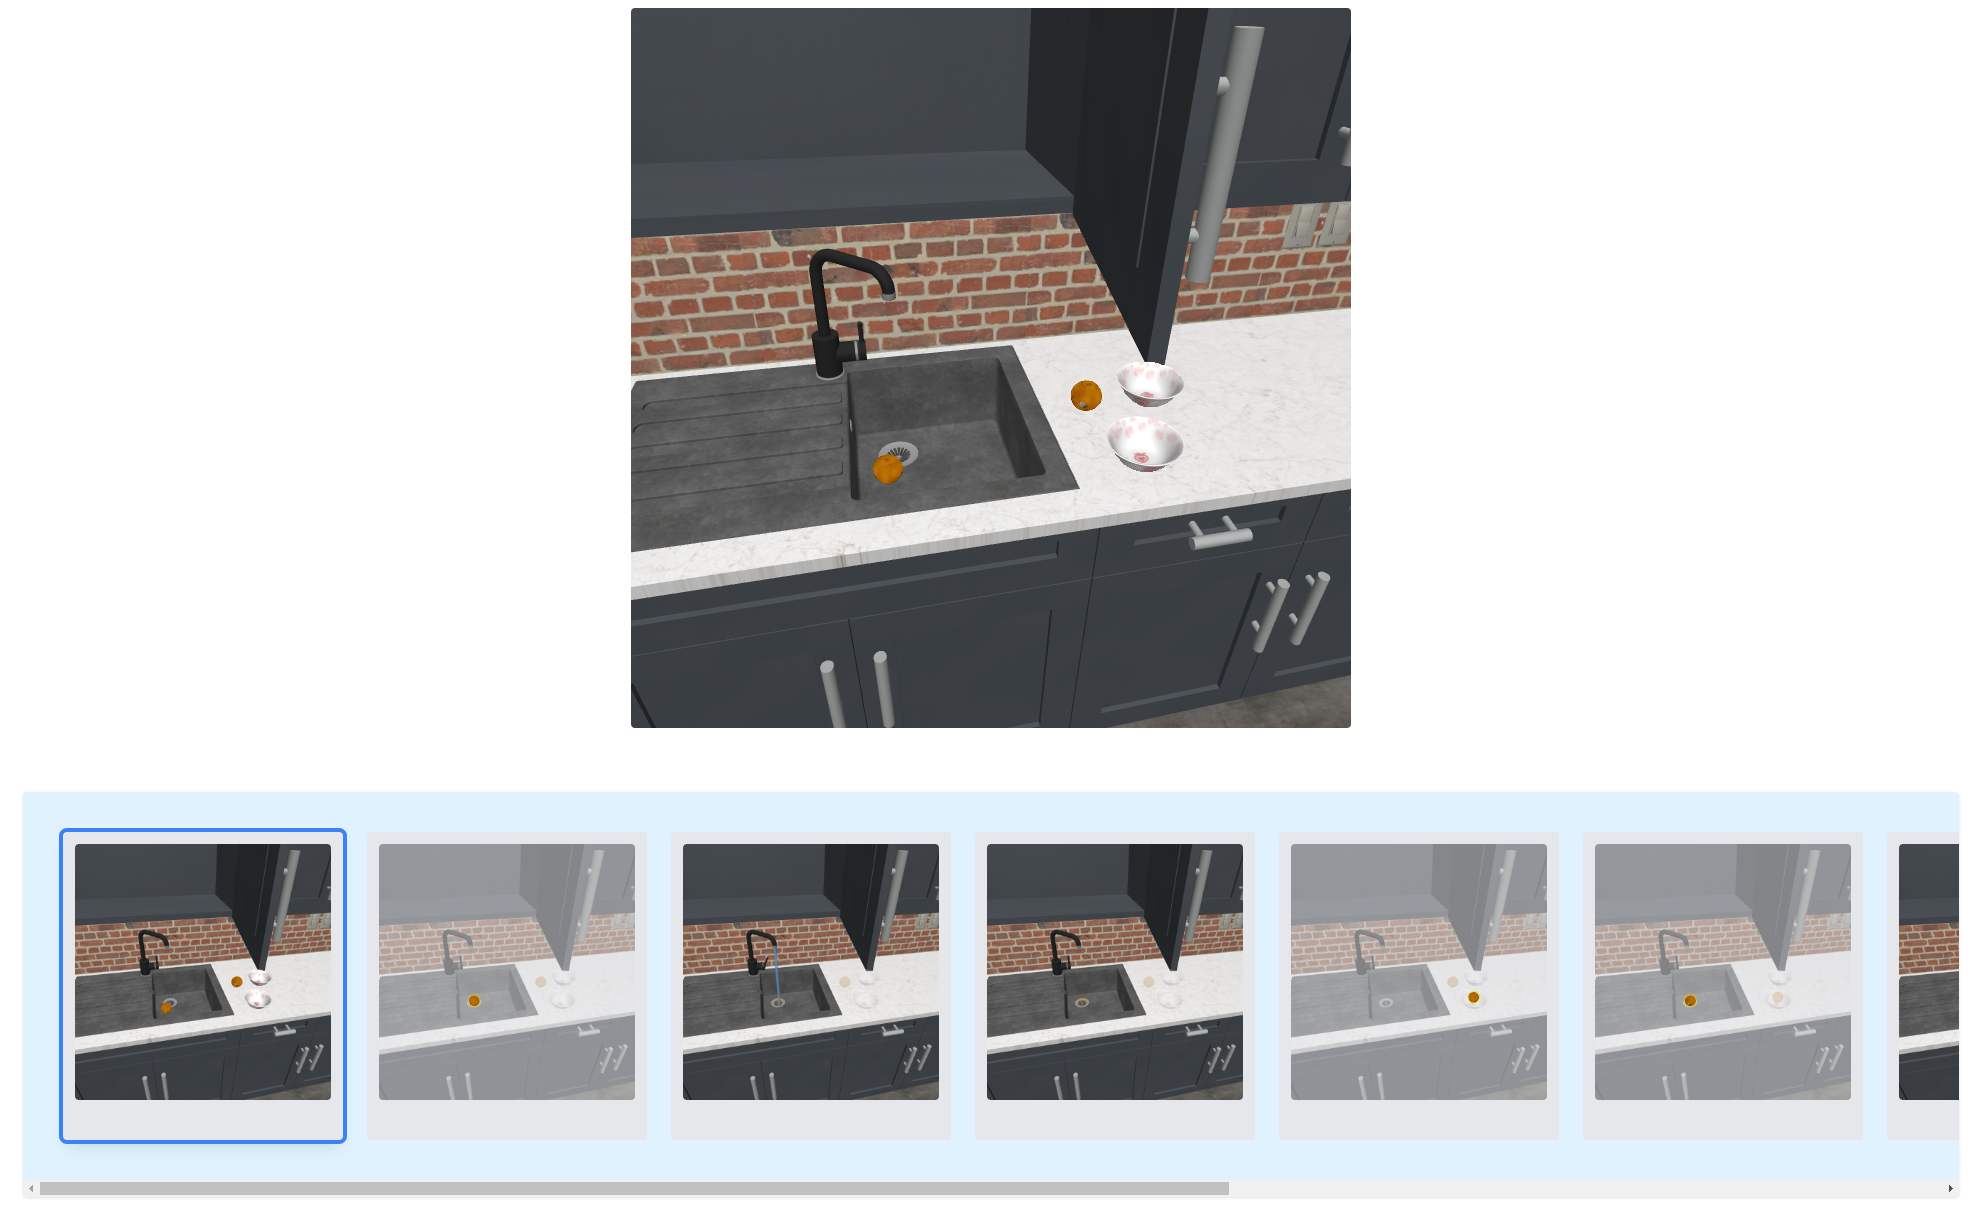
\includegraphics[width=0.8\textwidth]{figures/Interface.png}}
\caption{\projname's user interface, consisting of an editor (top) and a timeline (bottom). The editor allows users to manipulate objects and fixtures in the environment, while the timeline displays the current state of the environment and the desired changes.}
\label{fig:interface}
\end{figure*}

\section{Implementation}
\noindent \emph{High-level system design.} \projname consists of two major components: a back-end server that manages models to generate the image representations for manipulation and enables features such as automatic captioning, and a user interface for viewing and editing the images, enabling users to create robot instructions. The server is realized as a Flask application that enables two-way communication between the models and the interface. The models are hosted as TCP sockets on workstations within the local network and communicate with the Flask server to respond to requests from the interface. The user interface is built using ReactJS. Our implementation for the user study utilizes images from kitchen environments created using Robocasa~\cite{nasiriany2024robocasa}. 

%% Python (Flask) + ZMQ + ReactJS

\subsection{Representing the robot's environment} 
\projname creates an initial representation of the robot's environment by extracting information about the objects and fixtures present in them. 

\noindent \emph{Background image generation.} \projname assumes access to a predefined list of plausible objects and fixture states within the environment (e.g., a drawer being able to open or close) as well as the initial state of all fixtures. These assumptions are justified, as any robot entering a new environment would undergo an initialization phase to understand its surroundings. However, this knowledge can also be provided by the user or inferred by other models. Using this knowledge, \projname is able to enumerate all possible states of the environment. Each combination of states is then used to generate a background image that represents the environment in that state. For instance, in a kitchen environment consisting of a drawer and a cabinet, one combination of states could be the drawer being open and the cabinet being closed. Each of these images can be generated using a variety of methods. 

We experimented with fine-tuning language-conditioned diffusion models~\cite{brooks2023instructpix2pix, black2023zero} to generate images representing the appropriate state change but found the quality of the generated images to be inconsistent. Instead, for our prototype used in the user study, we utilized GPT-4o to generate code to modify the state of the fixtures inside the Robocasa environment. We envision that this could be plausible in the future given that many existing applications of robots assume the existence of digital twins~\cite{li2024evaluating}. At the end of this process, \projname creates a background image for all possible states, and sets the background image to the one that represents the current state.

\noindent \emph{Generating interactable objects and fixtures.} In order to enable the direct manipulation of images, \projname begins by detecting items from the previously known plausible list of items. In our physical robot implementation, the list of plausible items can be determined by prompting GPT-4o. Next, \projname generates bounding boxes for any detected items using an open vocabulary object detector, OWLv2~\cite{minderer2024scaling}. Then, information about the detected objects are passed to a segmentation model, Segment Anything (SAM~\cite{kirillov2023segment}), to generate manipulable masks. For the user study prototype, objects can be hidden when generating the background image so there is no white space and direct manipulation is possible at this stage. However, for the physical robot implementation, \projname performs an inpainting step to eliminate white spaces behind the objects before the user manipulates them~\cite{suvorov2022resolution}. For detected fixtures, \projname generates interactable regions by creating bounding boxes around the fixtures and enabling mouse clicks within these regions to activate state changes. 

\noindent \emph{Initializing the environment and state.} Upon generating backgrounds as well as representing objects and fixtures, the server transmits this information to the user interface. The environment describes static information about the environment, such as the background image and the interactable regions, while the state describes the current state of the environment. Once this information is received, the user interface renders the initial state of the environment as a step in the timeline represented as an SVG image.

\noindent \emph{Manipulating environment state.} The user can interact with the environment by manipulating objects and fixtures. Each time a new step is created, a new environment state is generated by copying the previous step and updating the data about any objects that moved or fixtures that changed state. When the user interacts with the interface, the system creates a new step by copying the representation of the previous step while updating data about any objects that moved. 

% After processing the initial state of all fixtures, the background image, generated masks, and bounding boxes for the fixtures are sent to user interface and rendered as a an SVG image inside a step. When the user clicks the initial step, the underlying representation is rendered inside an image editing application (\mk{CITE website}). The editor enables simple interactions such as the selection, deselection, and manipulating individual objects. When the user performs direct manipulations on one or more objects, the system creates a new step by copying the representation of the previous step while updating data about any objects that moved. To enable interactable fixtures, bounding boxes containing the location of fixtures are utilized to detect mouse clicks within this region, which activates a state change. When changing state, the current state variable is updated and the corresponding background image is retrieved and utilized when creating the step.

\noindent \emph{Predicting future steps (autocomplete)}

%Before the user begins providing instructions to the robot, \projname creates this initial representation to represent all objects and fixtures that are present in the environment, and determines the initial state. We assume access to the initial state of fixtures in the environment, such as the presence and number of cabinets, drawers, and sinks. For instance, a sample initial state could 


%This step can either be performed manually by a user when introducing their robot to their home, or automatically using models. 



% Describe how we make this by enumerating states 

% Sim/Susie/GPT

% How we make masks

% How we make interactable regions
